%% Combine this two slides into one 

\frame{ 
    \frametitle{Liquid Chromatography (LC)}
    \framesubtitle{A method to reduce sample complexity when analyzing molecular mixtures.}
    
\only<1>{
\begin{figure}[c]
    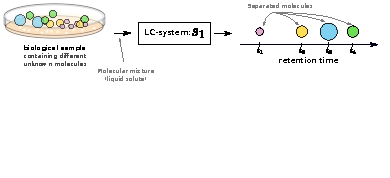
\includegraphics[width=\textwidth]{images/lc_separation_1.pdf}
\end{figure}
}
\only<2>{
\begin{figure}[c]
    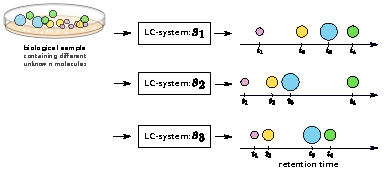
\includegraphics[width=\textwidth]{images/lc_separation_2.pdf}
\end{figure}
}
\vspace{-0.4cm}
\visible<2>{
\begin{small}
\begin{alertblock}{Observations}
\vspace{-0.25cm}
\begin{itemize}
    \item Retention time of a molecule varies across chromatographic system.
    \item \emph{Retention orders} are preserved.
\end{itemize}
\end{alertblock}
\end{small}
}

}

% \frame{
%     \frametitle{Retention times (RTs) for metabolite identification} 
%     
% \begin{itemize}
%      \item Retention times are \emph{valuable} orthogonal information \cite{Ruttkies2016,Stanstrup2015,Aicheler2015} \hfill\ex{distinction of diastereoisomers}
%      \item State-of-the-art machine learning metabolite identification methods use \emph{only} MS/MS information \cite{Brouard2016,Duehrkop2015} 
% \end{itemize}
% 
% \begin{alertblock}{Challenges utilizing RTs}
% \begin{enumerate}
%     \item Measurements are \emph{LC-system specific}. 
%     \item Public datasets are relatively \emph{small} and originate from \emph{heterogeneous systems}
% \end{enumerate}
% \end{alertblock}
% }

\frame{
    \frametitle{Utilizing retention times}
    
\begin{itemize}
    \item Retention times are \emph{valuable} information. \\
    \hfill \ex{Used to identify unknown molecular structures.}
    \item Huge number of methods to predict retention times exist.
    \item Suffer from the different retention times across systems.
\end{itemize}   

\begin{block}{We propose:}
\begin{itemize}
    \item \textbf{Predict the pairwise retention order} given molecular structures using preference learning.
    \item Prediction model can be trained on \emph{multiple} retention time datasets arising from \emph{heterogeneous} LC-systems. 
    \item Retention orders are largely preserved across LC-systems \cite{Stanstrup2015}.
\end{itemize}
 
\end{block}

}
